\section{Ejecución de pruebas}
Esta sección describirá las pruebas que se han realizado a las distintas propuestas de mejora del sistema. Primero se detallará el entorno de pruebas en el que han sido ejecutadas, el cual es reproducible, y posteriormente se comentarán los resultados obtenidos.

\subsection{Entorno de pruebas}
Las pruebas han sido realizadas en un entorno JIRA con varios proyectos: GPT4, que contiene incidencias ficticias y varios proyectos reales de la empresa LKS Next-GobTech, que, en el momento de realización de las pruebas siguen en desarrollo y son actualizados diariamente, pero que, por motivos de confidencialidad, no podrán ser revelado. En concreto, se ha realizado sobre 4 proyectos distintos, expuestos en la tabla \ref{tab:proyectos}.

\begin{table}[h]
\centering
\begin{tabular}{|c|c|c|}
\hline
\textbf{Proyecto} & \textbf{Nº de Incidencias} & \textbf{Nº de Personas} \\
\hline
GPT4 & 30 & 2 \\
\hline
MFM & 130 & 7 \\
\hline
JIRAGPT & 11 & 2 \\
\hline
INGURU & 129 & 5 \\
\hline
\end{tabular}
\caption{Número de incidencias y personas por proyecto.}
\label{tab:proyectos}
\end{table}

Los modelos de lenguaje utilizados serán GPT-3.5-turbo, el modelo base de OpenAI, que es barato y rápido y GPT-4o, el más avanzado modelo de OpenAI a fecha de realización del trabajo~\cite{gpt4o}. Las preguntas utilizadas se encuentran en el anexo I en forma de tabla, con su respectivo JQL esperado.

En cuanto a los resultados, se utilizará el conjunto de 100 preguntas creado durante la realización del trabajo, que contiene una variedad de preguntas de distinta dificultad y con la intención de cubrir la mayor cantidad de casos posibles, se considerará correcta una respuesta si las incidencias devueltas por la API de Jira con la sentencia JQL generada por el modelo son exactamente las mismas que las esperadas, que serán obtenidas mediante otra llamada a la API de Jira con la sentencia JQL predefinida que corresponde a la pregunta.

Los resultados consistirán en una puntuación del 0 al 1, que indicará el número de preguntas respondidas de manera correcta.

\subsection{Resultados}
Los resultados obtenidos, evaluados tanto para GPT-3.5-turbo como para GPT-4o se muestran a continuación, en las figuras \ref{fig:resultados_gpt35} y \ref{fig:resultados_gpt4o}, respectivamente. Se dividen en dos gráficas distintas, las cuales muestran el estado inicial, que es la ejecución sin ningún sistema de RAG y las tres propuestas de mejora:

\begin{figure}[H]
    \centering
    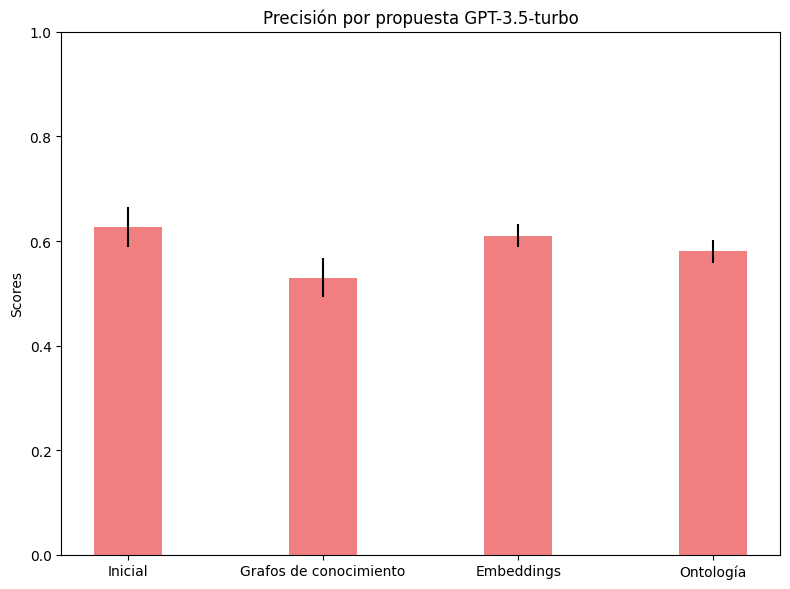
\includegraphics[width=0.65\textwidth]{images/Resultados_gpt35.png}
    \caption{Resultados para GPT-3.5-turbo}
    \label{fig:resultados_gpt35}
\end{figure}

\begin{figure}[H]
    \centering
    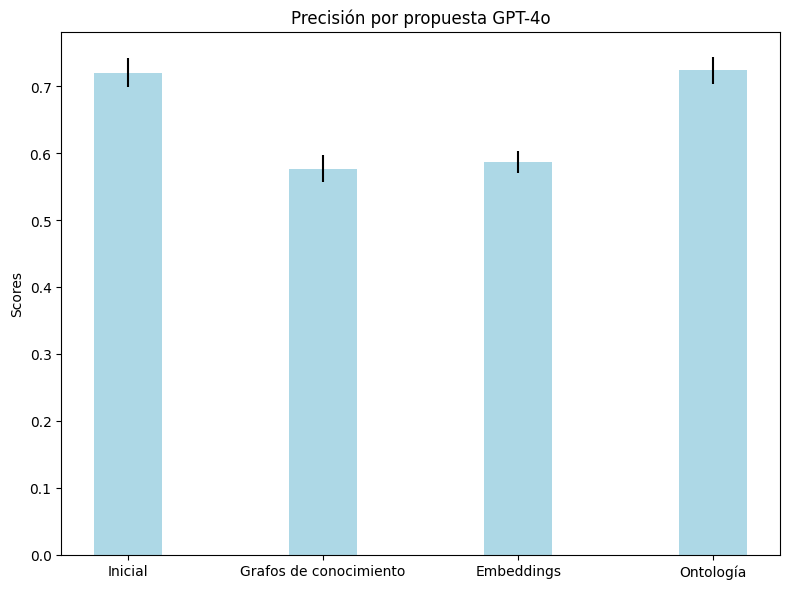
\includegraphics[width=0.65\textwidth]{images/Resultados_gpt4o.png}
    \caption{Resultados para GPT-4o}
    \label{fig:resultados_gpt4o}
\end{figure}

En las tablas se puede apreciar como la mejora en el modelo GPT-3.5 es mayor que en el modelo GPT-4o. Partiendo de la precisión inicial de 0.49 de GPT-3.5 sin técnicas de RAG, la arquitectura utilizada en el trabajo de Joel García, se incrementa hasta 0.57 con la propuesta de embeddings y 0.61 con la propuesta de la ontología, esto supone un aumento de alrededor de 10 puntos porcentuales si se usa la media de ambos. En el caso de GPT-4o, la precisión inicial es de 0.68, y se incrementa hasta 0.7 con la propuesta de embeddings y 0.72 con la propuesta de la ontología, lo que supone un aumento de 3 puntos porcentuales si se toma la media como medida. En ambos casos, la propuesta de la ontología resulta ser la que mejores resultados genera, aunque en el caso de GPT-4o, la mejora es menor que en el caso de GPT-3.5.

En cuanto a la mejora individual de cada una de las propuestas, tanto la opción de la ontología como la de los embeddings supone una mejora en precisión, mientras que la propuesta de los KGs reduce la precisión. Esto puede deberse a que, tanto la ontología como los embeddings, describen un concepto como JQL y aportan contexto sobre cómo crear este tipo de consultas, mientras que la opción de los KGs aporta datos sobre las incidencias de Jira, lo que requeriría que el modelo de lenguaje infiriese cómo funcionan las consultas JQL o la estructura de los proyectos de la empresa para poder generar consultas que sean acordes a ello, lo cual puede ser más complicado.

La diferencia entre la ontología y los embeddings es la manera en la que se representa la información de JQL, mientras que en la ontología se representa como las reglas haciendo uso de la representación semántica de una ontología, en los embeddings se representa como una serie de ejemplos de la documentación que se tratan de relacionar con la pregunta del usuario. La ontología por ende, parece ser una representación más adecuada para el problema, ya que la semántica de las reglas de JQL se puede llegar a expandir con una mayor cantidad de información y se puede explotar aún más la semántica de la ontología para mejorar la generación de consultas JQL.

Si miramos el grano fino, hay preguntas que el modelo nunca hace correctamente si no es aportado contexto, como por ejemplo `Muestra las incidencias que se han pasado de horas y por cuánto `. Esta pregunta el modelo la resuelve con el JQL 'timespent > originalestimate', lo cual, si no existe un campo 'originalestimate', no da resultados. Sin embargo, haciendo uso de la ontología, suele responder con 'workratio > 100', que es una respuesta que da resultados en cualquier caso. En el caso de los embeddings y el KG, no suele ser capaz de responderla de manera correcta tampoco.

El tipo de consultas que más complejas resultan para el modelo suelen ser las que esperan JQL que hace uso de 'CHANGED TO <Estado> DURING', ya que el modelo no parece conocer este tipo de uso. Al tener LKS Next-GobTech una serie de estados para las incidencias que son definidos por ellos mismos, como 'Aprobada', 'En Progreso', 'Validada' etcétera, hay preguntas que requieren hacer uso de este tipo de consulta JQL, como por ejemplo '¿Qué incidencias fueron resueltas durante mayo de 2024?', que necesitaría una consulta JQL como 'status CHANGED TO Resuelta DURING (2024-05-01,2024-05-31)' ya que lo que se busca son las incidencias que han cambiado al estado 'Resuelta', pero el modelo suele responder con 'status = 'Resuelto' AND resolved >= '2023-08-01' AND resolved <= '2023-08-31', que no devuelve las mismas incidencias. Esto con el uso de las ontologías parece mejorar, pero no de manera significativa, a veces usa este tipo de consultas, pero sigue comentiendo errores. De cara a una mejora del sistema, se podría buscar una manera de que el modelo aprenda este tipo de consultas, ya que parece ser un punto débil en la generación de consultas JQL.

Otro tipo de incidencias que el modelo falla la mayoría de intentos cuando se ejecuta sin contexto son las que piden incidencias con una prioridad concreta, por ejemplo, si se piden las incidencias de máxima prioridad, el modelo suele responder con 'priority = 'Máxima', que devuelve un error, ya que la prioridad es un campo fijo de Jira que utiliza 5 valores en inglés: 'Lowest', 'Low', 'Medium', 'High' y 'Highest', al ser preguntado en español y los campos ser palabras en inglés, parece confundirlo. Cuando se aporta contexto, principalmente la ontología, ya que se definen explícitamente los niveles de prioridad en esta, suele cometer menos fallos, pero no siempre acierta, a veces no parece querer aprovechar el contexto proporcionado por la ontología.

En el caso de grafo no se expone explícitamente ningún operador ni campo JQL, por lo que preguntas que el modelo base falla por no utilizar un campo concreto, como 'workratio', las falla también. El modelo además, parece confundir más los campos y operadores y no parece ser capaz de inferir cómo es la estructura de la información de Jira de LKS Next-GobTech.